\documentclass[11pt]{article}
\usepackage[margin=1in]{geometry}
\usepackage{amsmath,amssymb,booktabs,graphicx,float,array,xcolor}
\usepackage[hidelinks]{hyperref}
\usepackage{caption}
\captionsetup{font=small}
\setlength{\parskip}{4pt}
\setlength{\parindent}{0pt}
\newcommand{\thw}{\tilde\theta}

\title{COSC 527 Homework 2: Building and Verifying a Tabular RL Agent}
\author{Joshua Stenger}
\date{\today}

\begin{document}
\maketitle

\noindent All numbers below are printed by the submitted scripts and saved under
\texttt{results/}; figures are produced by \texttt{stenger\_hw2\_experiment.py}.
The professor-supplied \texttt{futura\_env/furuta\_env.py} is used \emph{exactly as
supplied}: no edits, no wrapper. Where the supplied environment differs from the
assignment text, this report states the difference rather than patching it.

%==========================================================================
\section{Environment and episode logic (\texttt{stenger\_hw2\_test\_environment.py})}

\textbf{Initial state.} With \texttt{FurutaEnv(seed=7)}, \texttt{reset()} returned
\[
x_0=[\phi,\dot\phi,\theta,\dot\theta]^T=[0.00500,\ 0,\ 0.01589,\ 0]^T .
\]
The arm is $0.29^\circ$ from its zero position, the pendulum is $0.91^\circ$ from
\emph{upright}, and both joints are at rest. The supplied \texttt{reset()} draws
$\phi_0,\theta_0\sim U(-0.02,0.02)$~rad: it starts every episode near the
\emph{upright} equilibrium, not the downward one. The time step is
$\Delta t=0.01$~s and \texttt{max\_steps}$=2000$ (20~s).

\textbf{Actions.} Applying each action from the same state and reading
\texttt{info["torque"]}:
\begin{center}
\begin{tabular}{lccc}\toprule
Action index & 0 & 1 & 2\\\midrule
Motor torque (N\,m) & $-0.02$ & $0.00$ & $+0.02$\\\bottomrule
\end{tabular}
\end{center}
Any other index raises \texttt{ValueError}.

\textbf{Sampled transition.} From $S_t=x_0$ with $A_t=2$ ($+0.02$~N\,m):
$R_{t+1}=0.99801$ and
$S_{t+1}=[0.00555,\ 0.10831,\ 0.01556,\ -0.06538]^T$
(\texttt{terminated=False}, \texttt{truncated=False}). The positive torque
accelerates the arm ($\dot\phi>0$) and the reaction tips the pendulum the
other way ($\dot\theta<0$). The reward is $1-(\theta/0.349)^2-0.001\tau^2$.

\textbf{Episode outcomes.} I read these from \texttt{step()} and checked each one:
\begin{center}
\small
\begin{tabular}{p{2.6cm}p{5.6cm}p{6.4cm}}\toprule
Outcome & Supplied environment rule & Observed\\\midrule
Unsafe termination & \texttt{terminated=True} if $|\theta|>20^\circ$ \emph{or} $|\phi|>\pi$; reward $=-10$ &
zero torque from \texttt{reset()}: ends at step 55 (0.55~s), $\theta=20.41^\circ$, $R=-10$;
arm started at $\phi=\pi-0.001$, $\dot\phi=1$: ends in 1 step, $R=-10$\\
Time-limit truncation & \texttt{truncated=True} when \texttt{steps}$\ge$\texttt{max\_steps} &
exact upright equilibrium, \texttt{max\_steps}$=50$: \texttt{terminated=False}, \texttt{truncated=True} at step 50\\
Success & \emph{none}: \texttt{info} only holds \texttt{torque, theta, phi} &
the 5~s objective must be measured by the analysis code (500 consecutive steps with $|\thw|\le20^\circ$)\\\bottomrule
\end{tabular}
\end{center}
Truncation is not a terminal state. My TD update therefore still bootstraps on a
truncated step and zeroes the continuation only when \texttt{terminated} is true.

\textbf{Is being outside the upright region terminal?} The assignment says it
should not be, but in the supplied environment \emph{it is}. Starting from the
hanging state $[0,0,\pi,0]$, the first \texttt{step()} returns
\texttt{terminated=True} with $R=-10$. The test also uses the raw angle rather
than $\mathrm{wrapToPi}(\theta)$, so $\theta=2\pi$ (physically upright,
$\thw=0$) is also terminated with $R=-10$.

This termination rule makes swing-up impossible. A swing-up trajectory must start
at $|\thw|=\pi$ and pass through every angle between $\pi$ and $20^\circ$ before
it reaches the balancing region. If every state outside $\pm20^\circ$ ends the
episode, then from a downward start every episode lasts exactly one step and
returns $-10$. The agent never observes a state on the swing path. Every TD target
for those states is the terminal value $-10$ with zero continuation, so no action
looks better than any other and nothing can ever propagate value back from the
upright region. Because the environment may not be modified, the experiment in
Section~5 is the \emph{balancing} task the supplied code implements (start near
upright, keep $|\theta|\le20^\circ$). The 5~s objective is still evaluated
exactly as specified.

%==========================================================================
\section{State discretization (\texttt{stenger\_hw2\_state\_discretization.py})}

Bins are internal edges passed to the supplied \texttt{discretize\_state}
(\texttt{np.digitize}); $k$ edges give $k+1$ bins. $\theta$ is wrapped with
$\mathrm{wrapToPi}$ first.

\begin{center}
\small
\begin{tabular}{cp{4.3cm}cp{6.4cm}}\toprule
Variable & Selected range / internal edges & Bins & Reason for the choice\\\midrule
$\phi$ & $[-1,1]$ rad; $\{-1,-0.5,0,0.5,1\}$ & 6 &
random play kept $|\phi|<0.5$; finer bins near 0, outer bins warn of drift toward the $\pm\pi$ arm limit\\
$\dot\phi$ & $[-3,3]$ rad/s; $\{-3,-1.5,0,1.5,3\}$ & 6 &
max $|\dot\phi|$ under random play was 2.6 rad/s; sign of arm velocity matters most\\
$\thw$ & $[-20^\circ,20^\circ]$; $\{\pm20,\pm10,\pm5,\pm2,0\}^\circ$ & 10 &
the env terminates outside $\pm20^\circ$, so 8 bins resolve the live region (finest near upright); the two open outer bins cover the rest of $[-\pi,\pi]$\\
$\dot\theta$ & $[-3,3]$ rad/s; $\{\pm3,\pm1.5,\pm0.5,0\}$ & 8 &
max $|\dot\theta|$ under random play was 3.3 rad/s; finer near 0 where balancing corrections happen\\\bottomrule
\end{tabular}
\end{center}

\[
|\mathcal S| = 6\cdot6\cdot10\cdot8 = 2880,\qquad |Q|=|\mathcal S|\,n_a=2880\cdot3=8640 .
\]
The flat row index is \texttt{np.ravel\_multi\_index(bins, (6,6,10,8))}.

\begin{table}[H]
\centering\small
\begin{tabular}{lll c r}\toprule
Test & State $[\phi,\dot\phi,\theta,\dot\theta]$ & $\thw$ & Bins & Index\\\midrule
Upright, at rest & $[0,0,0,0]$ & $0$ & $(3,3,5,4)$ & 1724\\
Downward, at rest & $[0,0,\pi,0]$ & $\pi$ & $(3,3,9,4)$ & 1756\\
$\theta$ near $-\pi$ & $[0,0,-\pi+0.01,0]$ & $-3.1316$ & $(3,3,0,4)$ & 1684\\
$\theta$ near $+\pi$ & $[0,0,\pi-0.01,0]$ & $3.1316$ & $(3,3,9,4)$ & 1756\\
$\theta=3\pi/2$ (wraps) & $[0,0,4.7124,0]$ & $-\pi/2$ & $(3,3,0,4)$ & 1684\\
$\dot\phi$ on edge & $[0,1.5,0,0]$ & $0$ & $(3,\mathbf 4,5,4)$ & 1804\\
$\theta$ on edge $+5^\circ$ & $[0,0,0.0873,0]$ & $5^\circ$ & $(3,3,\mathbf 7,4)$ & 1740\\
Velocities below range & $[0,-10,0,-14]$ & $0$ & $(3,\mathbf 0,5,\mathbf 0)$ & 1480\\
Velocities above range & $[0,10,0,14]$ & $0$ & $(3,\mathbf 5,5,\mathbf 7)$ & 1887\\
Typical balancing state & $[0.2,0.8,-0.05,-0.7]$ & $-2.9^\circ$ & $(3,3,3,2)$ & 1706\\\bottomrule
\end{tabular}
\caption{Discretizer tests (all indices lie in $[0,2879]$).}
\end{table}

\textbf{Out-of-range values and edges.} Only internal edges are stored, so the
first and last bins are open-ended. \texttt{np.digitize} returns 0 for any value
below the first edge and $k$ for any value above the last edge. Out-of-range
values (e.g.\ $\dot\theta=\pm14$) are therefore clamped to the extreme bin and
always give a valid index; they never raise an error. A value exactly on an edge
belongs to the upper bin (\texttt{right=False}): $\dot\phi=1.5$ goes to bin 4,
not 3. Angles near $\pm\pi$ fall in the two outer $\thw$ bins (0 and 9). These
are physically adjacent but are different table rows. That is harmless here
because both are terminal under the supplied environment. A verification script
also maps 2000 random states with components in $[-100,100]$ and confirms every
index is valid.

%==========================================================================
\section{$\epsilon$-greedy behaviour policy (\texttt{stenger\_hw2\_epsilon\_greedy.py})}

\textbf{Implementation and tie rule.} Draw $u\sim U(0,1)$. If $u<\epsilon$,
choose uniformly among \emph{all} $n_a=3$ actions, greedy actions included.
Otherwise choose uniformly among the actions whose value equals
$\max_a Q(s,a)$ (exact ties). The implied probabilities are
\[
P(a)=\frac{\epsilon}{n_a}+\frac{1-\epsilon}{|\mathcal G(s)|}\,\mathbb 1[a\in\mathcal G(s)],\qquad
\mathcal G(s)=\arg\max_a Q(s,a).
\]
For $Q(s^\dagger,\cdot)=[1,2,2]$, $\mathcal G=\{1,2\}$. With $\epsilon=0.2$:
$P(0)=0.2/3=0.0667$ and $P(1)=P(2)=0.0667+0.8/2=0.4667$. With $\epsilon=0$:
$[0,0.5,0.5]$. Random seed: \textbf{527} (\texttt{np.random.default\_rng(527)},
re-seeded for each $\epsilon$). I drew 10{,}000 samples, and the code asserts
that the Q table was unchanged afterwards.

\begin{table}[H]
\centering\small
\begin{tabular}{c ccc ccc c}\toprule
 & \multicolumn{3}{c}{Counts} & \multicolumn{3}{c}{Empirical / expected frequency} & Std.\ error\\
$\epsilon$ & $a{=}0$ & $a{=}1$ & $a{=}2$ & $a{=}0$ & $a{=}1$ & $a{=}2$ & (greedy)\\\midrule
0.20 & 658 & 4658 & 4684 & 0.0658 / 0.0667 & 0.4658 / 0.4667 & 0.4684 / 0.4667 & 0.0050\\
0.00 & 0 & 4986 & 5014 & 0 / 0 & 0.4986 / 0.5 & 0.5014 / 0.5 & 0.0050\\\bottomrule
\end{tabular}
\end{table}
Every empirical frequency lies within one binomial standard error
$\sqrt{p(1-p)/N}$ of the predicted value. The data rule out the two common
alternative implementations:
\begin{itemize}\itemsep0pt
\item exploration over \emph{non-greedy} actions only would give $P(0)=0.20$;
\item \texttt{argmax} tie-breaking would give $[0.067,0.867,0.067]$.
\end{itemize}
With $\epsilon=0$, action 0 is never chosen because it is not greedy. Actions 1 and
2 each appear about half the time because the exploitation branch still breaks the
tie at random. A greedy policy is therefore deterministic only when the maximum
is unique.

%==========================================================================
\section{SARSA and Q-learning update audit (\texttt{stenger\_hw2\_audit.py})}

Settings: $\alpha=0.1$ and $\gamma=0.9$. Q is filled with values drawn from
$U(0,5)$ (seed 4), rounded to 0.01, so next-state values are distinct. Both
transitions come from \texttt{FurutaEnv.step()}. All quantities are stored before
any update. The script then computes the result by hand and with the
\texttt{td\_update} function used in training, and asserts that the two agree
and that only $Q(S_t,A_t)$ changed.

\textbf{Nonterminal transition} (from \texttt{reset()} with seed 4, $A_t=2$):
\begin{center}\small
\begin{tabular}{ll}\toprule
$S_t$ & $[0.017722,\ 0,\ 0.000453,\ 0]$ $\to$ bins $(3,3,5,4)$, index 1724\\
$A_t$ & 2\\
$R_{t+1}$ & $0.9999995$\\
$S_{t+1}$ & $[0.018292,\ 0.113903,\ 0.000089,\ -0.072854]$ $\to$ bins $(3,3,5,3)$, index 1723\\
$A_{t+1}$ & 2 (an exploratory, non-greedy action)\\
$Q_{\text{old}}(S_t,A_t)$ & 4.57\\
$Q_{\text{old}}(S_{t+1},\cdot)$ & $[3.66,\ 4.08,\ 2.37]$\\\bottomrule
\end{tabular}
\end{center}
\begin{align*}
Y^{\text{SARSA}} &= 0.9999995 + 0.9\,Q(S_{t+1},2) = 0.9999995+0.9(2.37) = 3.1330,\\
Y^{\text{Q}} &= 0.9999995 + 0.9\max_a Q(S_{t+1},a)= 0.9999995+0.9(4.08) = 4.6720,\\
Q^{\text{SARSA}}_{\text{new}} &= 4.57+0.1(3.1330-4.57) = 4.4263,\qquad
Q^{\text{Q}}_{\text{new}} = 4.57+0.1(4.6720-4.57) = 4.5802 .
\end{align*}
The program printed $Y^{\text{SARSA}}=3.133000$, $Y^{\text{Q}}=4.672000$, and new
values $4.426300$ and $4.580200$, identical to the hand calculation.

\textbf{When the targets agree.} The two targets are equal whenever
$Q(S_{t+1},A_{t+1})=\max_aQ(S_{t+1},a)$, i.e.\ the behaviour policy chose a greedy
next action, which happens with probability $1-\epsilon+\epsilon/n_a$ for a unique
maximum. They are also equal on terminal transitions, where both continuations
are zero. They differ when $A_{t+1}$ is an exploratory non-greedy action, as here:
SARSA (on-policy) evaluates the action actually taken and is pulled down by it,
while Q-learning (off-policy) evaluates the greedy action no matter what
$A_{t+1}$ is.

\textbf{Terminal transition.} Start at $S_t=[0,0,19.9^\circ{=}0.34732,\,2.0]$
(index 1750) and apply $A_t=1$. The pendulum leaves the region:
$S_{t+1}=[-0.00034,-0.06844,0.36797\,(21.08^\circ),2.12990]$ (index 1198), with
\texttt{terminated=True} and $R_{t+1}=-10$. I deliberately set
$Q(S_{t+1},\cdot)=[100,200,300]$, with $A_{t+1}=2$ and $Q_{\text{old}}(S_t,A_t)=4.79$. Then
\begin{align*}
Y^{\text{SARSA}} &= -10 + 0.9\cdot\underbrace{0}_{\text{terminal}}\cdot 300 = -10,\qquad
Y^{\text{Q}} = -10 + 0.9\cdot 0\cdot\max(100,200,300) = -10,\\
Q_{\text{new}} &= 4.79+0.1(-10-4.79) = 3.3110 \quad\text{(both methods; program: 3.311000)}.
\end{align*}
The large next-state values have no effect: the continuation is zero because the
transition is terminal, and the next-state row is never read.

%==========================================================================
\section{Preliminary learning experiment (\texttt{stenger\_hw2\_experiment.py})}

\begin{center}\small
\begin{tabular}{ll}\toprule
Algorithm & Q-learning (off-policy TD control)\\
Episodes per seed & 1500\\
Step size $\alpha$ / discount $\gamma$ & 0.1 / 0.99\\
Exploration & $\epsilon$-greedy, linear decay $1.0\to0.05$ over episodes 0--1000, then held at 0.05\\
Q-table initialization & all zeros, $2880\times3$\\
Training seeds & 0, 1, 2 (environment \texttt{FurutaEnv(seed)} and agent RNG)\\
Evaluation & \texttt{reset} seed $10000+$training seed, Q frozen (read-only), $\epsilon=0$, no updates\\
Max episode duration & \texttt{max\_steps}$=2000$, $\Delta t=0.01$~s $\Rightarrow$ 20~s\\
Environment & supplied \texttt{FurutaEnv} defaults (reward, $\pm20^\circ$ / $\pm\pi$ limits, upright start)\\\bottomrule
\end{tabular}
\end{center}

\begin{figure}[H]
\centering
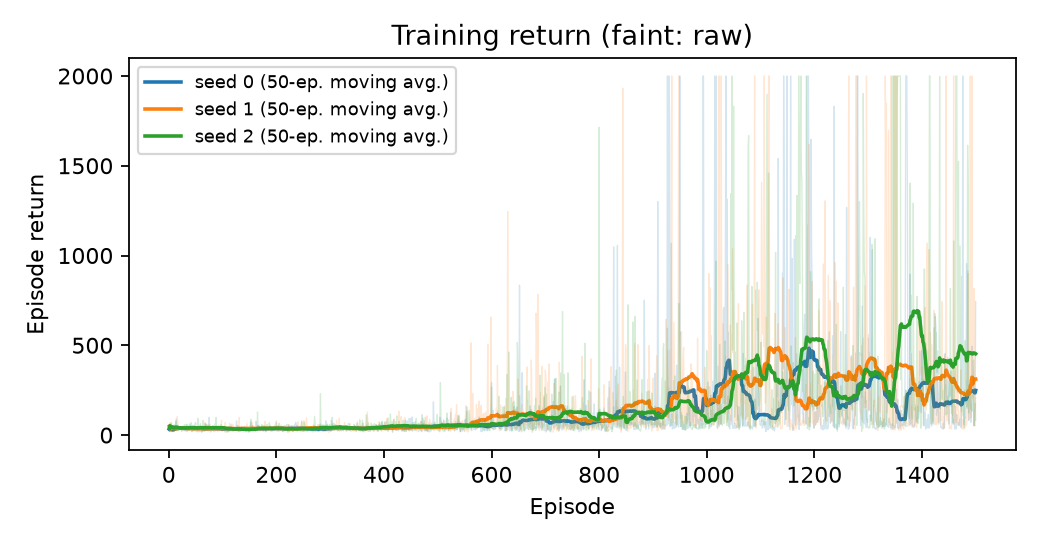
\includegraphics[width=0.49\linewidth]{figures/returns.png}\hfill
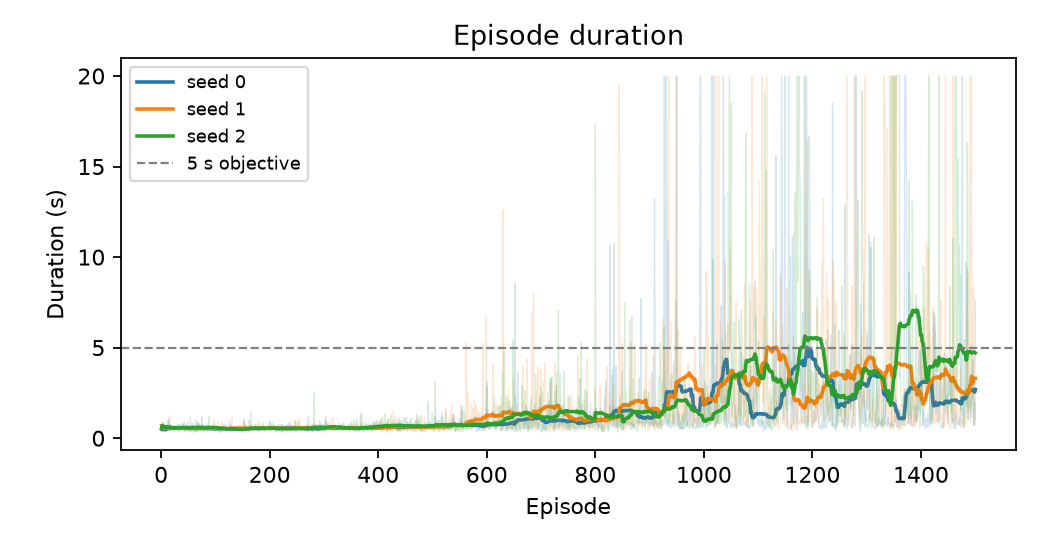
\includegraphics[width=0.49\linewidth]{figures/durations.png}\\[2pt]
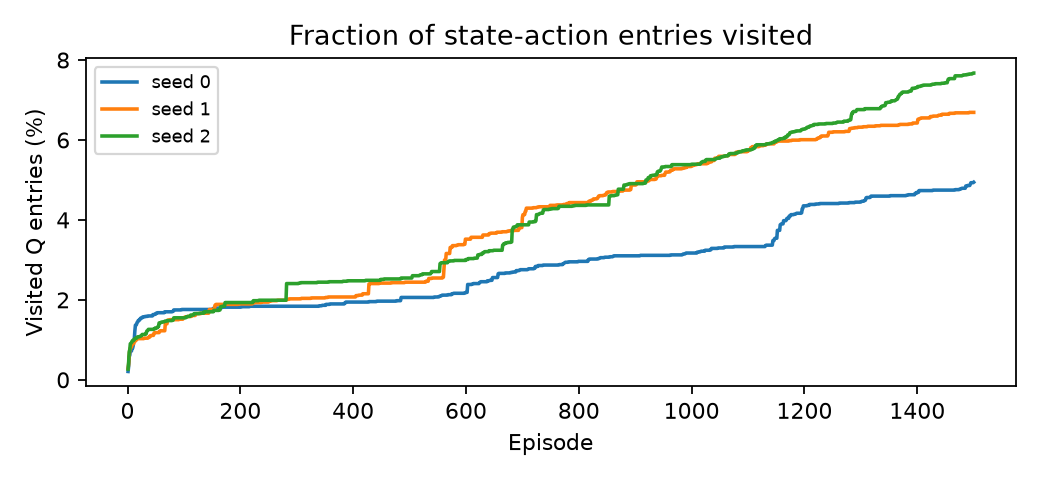
\includegraphics[width=0.49\linewidth]{figures/coverage.png}\hfill
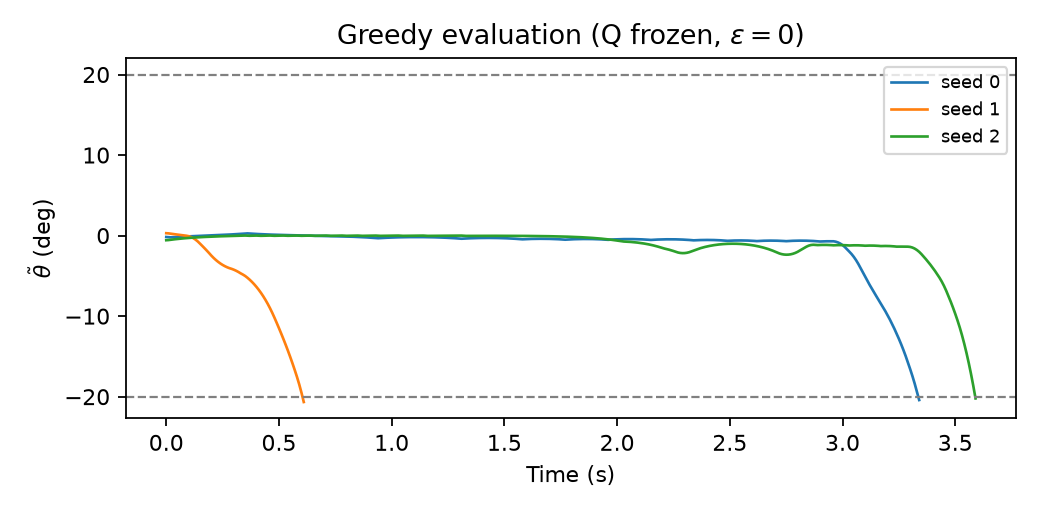
\includegraphics[width=0.49\linewidth]{figures/evaluation_theta.png}
\caption{Top: episode return (50-episode moving average; raw values faint) and
episode duration. Bottom left: fraction of the 8640 state-action entries visited
at least once. Bottom right: $\thw$ during one greedy evaluation episode per seed
(dashed lines: $\pm20^\circ$).}
\end{figure}

\begin{table}[H]
\centering\small
\begin{tabular}{lccc}\toprule
 & Seed 0 & Seed 1 & Seed 2\\\midrule
Mean return, first / last 100 episodes & 36.1 / 212.2 & 36.0 / 320.2 & 40.5 / 430.4\\
Mean duration, first / last 100 episodes (s) & 0.54 / 2.33 & 0.54 / 3.40 & 0.59 / 4.49\\
Training episodes lasting $\ge5$~s / reaching 20~s & 69 / 19 & 114 / 22 & 110 / 20\\
Visited Q entries at end & 4.9\% & 6.7\% & 7.7\%\\
Greedy evaluation: duration, outcome & 3.34~s, $|\theta|>20^\circ$ & 0.61~s, $|\theta|>20^\circ$ & 3.59~s, $|\theta|>20^\circ$\\
Greedy evaluation: longest run with $|\thw|\le20^\circ$ & 3.34~s & 0.61~s & 3.59~s\\\bottomrule
\end{tabular}
\end{table}

\textbf{Interpretation.} For roughly the first 500 episodes ($\epsilon>0.5$),
behaviour is close to random and episodes last about 0.55~s, the same as zero
torque. After that, durations and returns rise in all three seeds. Every seed
produced training episodes that balanced for the full 20~s, so the
representation can express a balancing controller. The greedy evaluation is less
good. Because of the supplied \texttt{reset()}, every evaluation episode
\emph{started inside the upright region}; it never had to swing up. The policy
held $\thw\approx0$ for about 3.3--3.6~s (seeds 0 and 2) or 0.6~s (seed 1), then
the pendulum fell past $20^\circ$. In the swing-up terms of the assignment, the
policy therefore did not remain near downward, did not generate a growing swing,
and did not need to reach the upright region (it started there). It
\textbf{did not complete the 5-second balancing objective} for any seed.

%==========================================================================
\section{Diagnostic reflection}

\textbf{(a) Most limiting component: the discretization.} During training, about
19\% of the last 500 episodes of seeds 1 and 2 lasted at least 5~s (at
$\epsilon=0.05$). Yet the greedy rollouts from the same tables lasted only
0.6--3.6~s, and seed 1 failed within 0.6~s. The greedy policy's quality depends
heavily on small differences in the start state, which points to aliasing. 75--79\%
of all visits fell into only the two $\thw$ bins within $\pm2^\circ$ of upright.
Those two bins merge many continuous states that need different torques, so one
greedy action per cell cannot be correct for all of them. The slow drift visible
before the fall (e.g.\ seed 2's arm reached $\phi=-1.08$~rad) is another symptom:
$\phi$ is resolved only in 0.5-rad steps, so the policy cannot see the drift until
it is large. The number of episodes is a secondary limit, since the curves are
still rising at episode 1500.

\textbf{(b) Rarely visited region: large pendulum velocity.} The outer
$\dot\theta$ bins ($|\dot\theta|>3$~rad/s) were visited only 3, 11 and 5 times
across about 225k--287k steps per seed. The outer $\thw$ bins (beyond $\pm20^\circ$)
are never acted from, because they are terminal. For balancing, I would
\emph{not} refine $|\dot\theta|>3$: states there almost always fall, and extra
bins would only add unvisited rows (2588--2697 of the 2880 rows were never
updated). I would instead move resolution inward, using more bins in
$|\thw|<5^\circ$ and $|\dot\theta|<1.5$ where nearly all decisions happen. For
the midterm swing-up (if the environment's termination rule allows it), the
opposite holds: the $\dot\theta$ range must grow to several rad/s and the
$\thw$ bins outside $\pm20^\circ$ become essential. They should then be split
so that $-\pi$ and $+\pi$ map to one physical region.

\textbf{(c) A test a return plot would hide.} The terminal-transition audit sets
$Q(S_{t+1},\cdot)=[100,200,300]$ and checks that the target is exactly
$R=-10$. If the code bootstrapped through terminal states, or zeroed the
continuation on \emph{truncation} instead of termination, the return curve would
still rise. Durations are driven by the same reward, so the bug would show up only
as subtly wrong values near the $\pm20^\circ$ edge. The assert-based script
\texttt{stenger\_hw2\_verification.py} also caught a real error during this
homework. My first edge test expected $\dot\phi=1.5$ in bin 3, but
\texttt{np.digitize} correctly returns bin 4 (edges are lower-inclusive). The
test was wrong, not the discretizer. No training plot would have revealed which
side of an edge a value lands on. Finally, the environment test in Section~1
showed that the supplied environment terminates outside the upright region. A
learning curve alone would have looked like an ordinary, slowly improving
balancing run and would never have shown that swing-up is unreachable.

%==========================================================================
\appendix
\section{Use of generative AI}

\textbf{Tool:} Claude Code (Anthropic, model Claude Opus 5.5).

\textbf{Prompts / questions submitted.}
\begin{itemize}\itemsep0pt
\item ``The assignment is at \ldots HW2\_Tabular\_RL\_Checkpoint.pdf \ldots the futura\_env folder is the
environment provided by my professor, do not change the environment, but change the pearce files to be
stenger and have the correct code needed \ldots Generate me a latex report named report.tex in a folder
named report.''
\item ``No you do not need a wrapper, we should not be wrapping or editing the environment in any way
shape or form. We have to use what we were given.''
\end{itemize}

\textbf{How the responses influenced the work.} The tool drafted the six
\texttt{stenger\_hw2\_*.py} scripts and the README, ran them, and drafted this
report from the printed results and saved JSON files.

\textbf{Suggestions verified, corrected, or rejected.}
\begin{itemize}\itemsep0pt
\item \emph{Rejected:} the tool first proposed wrapping \texttt{FurutaEnv} in a
``swing-up'' class that would start episodes downward and ignore the
$20^\circ$ termination. I rejected this because the supplied environment must be
used as given. The code instead calls \texttt{reset()}/\texttt{step()} directly,
and Section~1 reports the termination behaviour honestly.
\item \emph{Corrected:} the generated verification test expected
$\dot\phi=1.5$ in bin 3. Running it failed, and checking the edges showed that
\texttt{np.digitize} correctly gives bin 4. The test was fixed (Section~6c).
\item \emph{Verified:} the $\epsilon$-greedy probabilities were derived by hand
and matched against the 10{,}000-sample counts. Every TD target and update in
Section~4 was recomputed by hand and asserted equal to the program output.
\end{itemize}

\textbf{Portions assisted.} Code: all \texttt{stenger\_hw2\_*.py} scripts, the
README, and the plotting code. Report: drafting of all sections, including the
Section~6 reflection, from results produced by the submitted implementation.
\end{document}
